\documentclass[conference]{IEEEtran}
\IEEEoverridecommandlockouts
% The preceding line is only needed to identify funding in the first footnote. If that is unneeded, please comment it out.
\usepackage{cite}
\usepackage{amsmath,amssymb,amsfonts}
\usepackage{algorithmic}
\usepackage{graphicx}
\usepackage{textcomp}
\usepackage{xcolor}
%\usepackage{booktabs}
\usepackage{tabularray}
\usepackage{flushend}
\UseTblrLibrary{booktabs}
\def\BibTeX{{\rm B\kern-.05em{\sc i\kern-.025em b}\kern-.08em
    T\kern-.1667em\lower.7ex\hbox{E}\kern-.125emX}}
\begin{document}

\title{Data Collection in the Wild: Challenges and Solutions}

\author{
\IEEEauthorblockN{Péter Udvardy}
\IEEEauthorblockA{\small \textit{Alba Regia Technical Faculty} \\
\textit{Óbuda University}\\
\textit{Székesfehérvár, Hungary}\\
\textit{udvardy.peter@amk.uni-obuda.hu}
}
\and
\IEEEauthorblockN{Levente Dimen}
\IEEEauthorblockA{\small \textit{Department of Cadastre, Civil Engineering} \\
\small \textit{and Environmental Engineering} \\
\textit{1 Decembrie 1918 University}\\
\textit{Alba Iulia, Romania}\\
\textit{dimenlev@yahoo.com}
}
\and
\IEEEauthorblockN{Gergely Vakulya}
\IEEEauthorblockA{\small \textit{Alba Regia Technical Faculty} \\
\textit{Óbuda University}\\
\textit{Székesfehérvár, Hungary}\\
\textit{vakulya.gergely@amk.uni-obuda.hu}
}
}


\maketitle

\begin{abstract}

Extensive monitoring plays a key role in environmental protection. This task, however
has many issues to solve, communication and data collection being a difficult one.
This paper focuses to the challenges of observing hard-to-access areas, e.g.
such as forests and wetlands. The performance of the possible solutions for this problem
are compared, focusing to sensor networking and LPWAN technologies, and a drone based solution
will be proposed. The presented method offers a robust, and reliable, yet simple
data collection solution. The hardware and software architecture, the communication protocol
will be described and the estimated performance of the system is analyzed.


\end{abstract}

\begin{IEEEkeywords}
environment monitoring, data collecion, sensor network, drone technology
\end{IEEEkeywords}

\section{Introduction}

Sensor networks consist of nodes with sensing, processing and communication
capabilities. Their main application area is data collection, especially
on large areas or with large number of points. In most applications
the power sources of the devices are batteries, since the mains current
is not an option. As the continuous lifespan of such a network is
preferrably measured in years, but at least in months, the power
budget must be highly optimized.

One of the most promising classic sensor networking applications was monitoring
of remote, nonaccessible areas \cite{corke2010}, such as rainforests
\cite{wark2008, cama2013}, volcanos \cite{werner2006, song2009} or glaciers
\cite{martinez2004, martinez2005}. 

\section{Related work}

Most conventional senskr network based monitoring
systems use a base a mesh routing protocol to
send all measurement messages to a dedicated base
station. In a typical setup the sensor nodes have
a limited amount of power (most commonly batteries),
while the power source of the base is practically
unlimited (mains power solar energy). These protocols
often apply TDMA (Time Division Multiple Access),
which relies on a tight time synchronization.
In such a system each message is relayed through
multiple subsequent nodes, which means extra energy
consumption each time. Another less obvious
disadvantage is, that nodes closer to the base
relay more packets, thus they consume more energy.

Another possible approach is to use one of the
modern LPWAN protocols (e.g. LoRa or NBIoT).
First these solutions obviously requite a working
infrastructure. Second they are typically not
designed to transfer large amount of (measurement)
data.

\section{The proposed monitoring method}

\subsection{System architecture}

The architecture of the monitoring system consists of several independent
measuring nodes and a base station, which is attached to a drone, flying
over the measurement area at regular times, allowing to download the
collected data.

The sensor nodes do preprogrammed measurements and store the collected data
in flash memory. 

\subsection{The proposed communication protocol}

In the proposed monitoring system the data collector nodes have limited
energy (they are powered by batteries) similarly to regular sensor networking
applications. Using a mesh protocol to collect the measured data each message
would be sent by possibly many sensor nodes. The proposed protocol uses a star
topology instead, which requires to send each message only once, but on the
other hand it assumes direct connection (i.e. line of sight).
The speciality of the system is, that the base station is absent in the huge
majority of the time and present only occasionaly.

The goal of the proposed communication protocol is to detect the presence
of the base station and transfer the collected data when the conditions are
given. The sensor nodes don't necessarily hear each other, therefore collision
avoidance is the task of the base station.

The protocol utilizes the fast acknowledgements of the 802.15.4 MAC layer.
Instead of listening for some kind of beacon messages transmitted by the
base station, the sensor nodes emit \emph{hello} messages
regularly and wait for an \emph{ACK} message.
The time interval of the \emph{hello} messages is a design parameter of
the protocol.

The 802.15.4 ACK packet has 3 unused bits (see Fig. \ref{ack-packet}), which
are used to sign, when the actual data transfer process is possible.
Each of the 8 combinations can sign different waiting times. This way
the base station can spread the time slots of the nodes. The nodes turn off
their radio during waiting. Note that the nodes do not need to maintain tight
time synchronization, for this task.

During the actual data transfer each node dend send the
previously collected data divided into packets. Each packet is sent
tightly next to each other, with acknowledgements by the base station.


%timeslots for the sensor nodes by the gateway. The 3 bits
%can define 8 possible combinations, where the \emph{000} means an extended
%waiting time. Nodes received that bit combination will send another \emph{hello}
%message, when the 



\subsection{Sensor nodes}

The hardware of the sensor node is based on an Unicomp UCMote Proton B mote.
The base board has an 8-bit ATmega128RFA1 Soc as the main controller. The
microcontroller core is running at 16 MHz, with an approx. 4 mA current
consumption from 3.3 V. The microcontroller has different sleep modes,
and can be stopped from program execution. When stopped, the current consumtion
is reduced to the TODO range. Another important parameter is the wakeup time,
which is in the range of microseconds. The SoC contains a 2.4 GHz radio unit,
that supports the 802.15.4 range standard for low-power low-range communication.
This communication channel is used only during testing for debug purposes only,
for two reasons. First the the 2.4 GHz band is not suitable for the proposed
monitoring system because of the high absorption of. Second, the board has
only a low gain chip antenna connected of the Soc.

The main board contains an additional AT86RF212 radio chip, which operates in
the 868 MHz ISM band. This radio chip can be configured to use different
communication speeds from 20 to 1000 kbps according to the link conditions.
Depending on the communication bandwidth the receiver sensitivity can be as good as
-110 dBm. With the +10dBm maximum power output the achievable link budget can
reach 120 dB, which is well suits to the proposed system. This radio is connected to
an MMCX RF connector, which allows to connect a high gain external antenna.

Since the drone is located above the sensor nodes during the data download
process the usual quarter wave vertical antennas are not a good choice for
this purpose, given they have very low gain in axial direction. QFH antennas \cite{adams1974},
however have good overhead gain, therefore they are much more suitable for the
proposed system.

The power source of the proposed sensor node consists of 4 D type non-rechargeable
lithium batteries, providing 76000 mAh capacity at 3.6 V.

\begin{figure}[htbp]
	\centering
	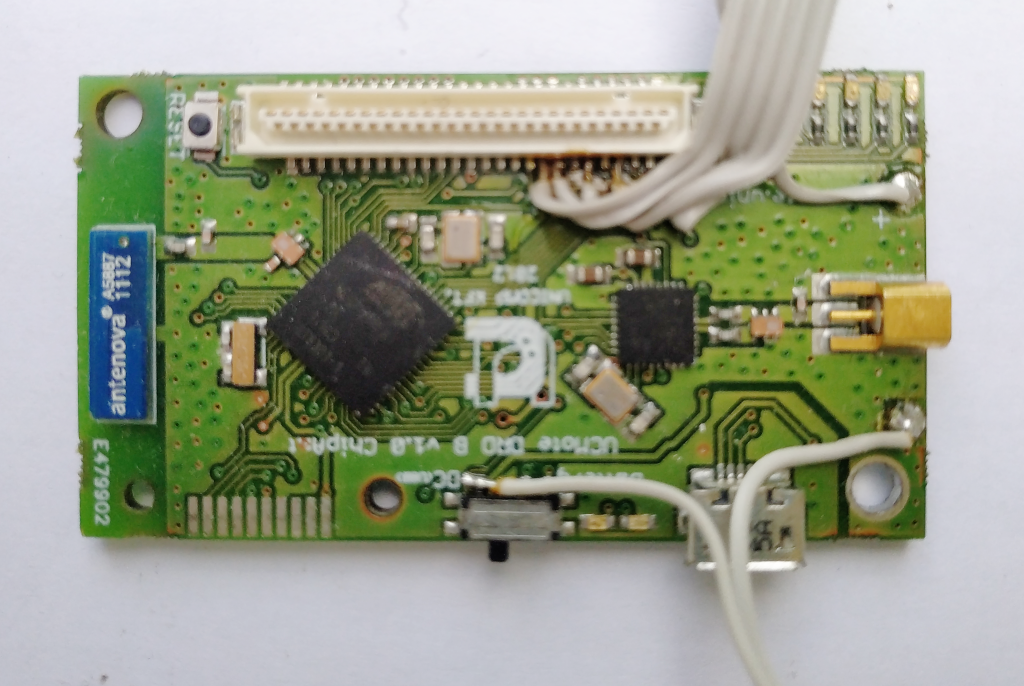
\includegraphics[width=0.35\textwidth]{fig/ucproton.png}
  \caption{The UCMote Proton B mote. }
	\label{fig-proton}
\end{figure}

The software of the sensor nodes is built around the TinyOS. It is a component
based real-time operating system, especially tailored for low-power
applications. It has support for different types of microcontrollers, radios
and sensors and the uniform interfaces make adding new device drivers and
communication protocols possible.

\cite{vakulya2013}

TinyOS already supported the ATmega128RFA1 SoC with its microcontroller core
and automatically put it in low-power mode, when it has no task to run and no
event to process. The 2.4 GHz radio is also supported and 802.15.4 standard
packets can be sent and received with a simple CSMA/CA MAC protocol. The other
radio chip (AT86RF212, 868 MHz) is also supported with the standard CSMA/CA
protocol, although the special low-power mode had to be implemented. To achieve this,
the header, which contains the source address, must be intercepted and the
time-critical background lookup must be processed in parallel with the recetion
of the remainig part if the packet, before the full packet arrives. Based on
the result of the lookup one of the reserved bits of the acknowledgement packet
is set of cleared, signaling the presence or the absence of a pending packet.

\begin{figure}[htbp]
	\centering
	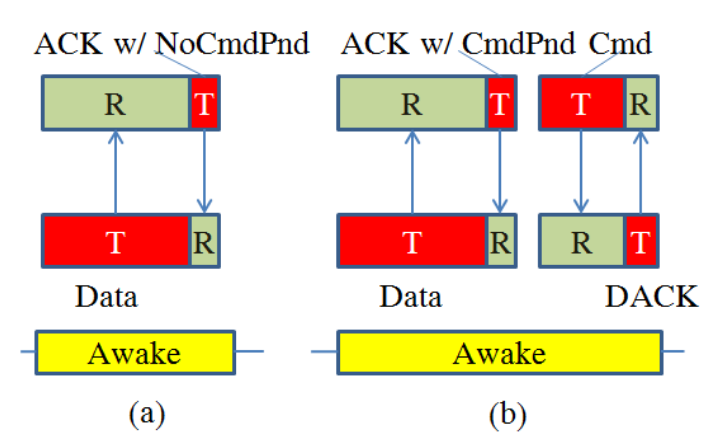
\includegraphics[width=0.35\textwidth]{fig/protocol.png}
  \caption{}
	\label{fig-piggyback}
\end{figure}

\section{Measurement scenarios}

\subsection{Low density environmental data collection}

In this scenario slowly changing environmental parameters are monitored. The sensor modalities are:

\begin{itemize}

  \item{Soil temperature with 16 bit resolution, one measurement every 5 minutes}
  \item{Air temperature with 16 bit resolution, one measurement every 5 minutes}
  \item{Ambient light intensity with 16 bit resolution, one measurement every 5 minutes}
  \item{Relative humidity with 8 bit resolution, hourly}
  \item{Soil moisture with 8 bit resolution, hourly}

\end{itemize}

A total of 15 sensor nodes are installed in the system.
In each node a total number of 1776 bytes are generated each day.
If the data is collected every two months, approx.
100 kBytes of data is fetched from each node. With a
pessimistic 20 kbps bandwidth approx 1 minute is
necessary to download this data amount from each node.
A 1 minute beacon interval for the sensor nodes would
give a good balance between latency and power
consumption. With these parameters the average flight
time can be estimated to approx. 20 minutes.

The 802.15.4 packet has a 13 byte header (including the preamble,
physical and MAC headers) and a 2 byte footer. With another
The length of a \emph{hello} message with a 5 byte payload is
20 bytes, which requires 8 ms to send with 20 kbps. The length of
the ACK packet is 11 bytes, which requires 4.4 ms of time.
Another approx. 1
ms is required to turn on and off the radio and approx. 2 ms
of gap time is required between the two packets. This adds up
to 15.4 ms. 
The actual data transfer requires approx. 60 seconds of time.
The on time of the radio can be calculated as follows for a year:

\begin{equation}
    T_{on,annual} = 60 \cdot 6 + 365 \cdot 24 \cdot 60 \ cdot \frac{15.4}{1000} = 8454 [s]
\end{equation}

Now the annual power consumption of the radio can be calculated as
follows:

\begin{eqnarray}
    C_{annual} &= T_{on,annual} * I_{radio,on} = \\
     &= \frac{8454 [s]}{3600} \cdot 20 [mA] = [mAh] = 47 [mAh]
\end{eqnarray}

Considering only the radio communication one D type cell would last for
several years (practically the self-discharge limits the lifespan).

\section{Summary}

In this paper 

\bibliographystyle{IEEEtran}
\bibliography{IEEEabrv,references}

\end{document}
